\documentclass[a4paper,14pt]{extarticle}

\usepackage[a4paper,top=20mm,bottom=20mm,left=30mm,right=10mm]{geometry}
\usepackage[T1,T2A]{fontenc}
\usepackage[utf8]{inputenc}
\usepackage[russian]{babel}
\usepackage{indentfirst}
\usepackage{titlesec}
\usepackage{graphicx}
\usepackage{verbatim}
\usepackage{fancyvrb}

\renewcommand{\baselinestretch}{1.3}

\setlength{\parindent}{12.5mm}
\titleformat{\section}{\normalsize\bfseries}{\indent\thesection}{1em}{}
\titleformat{\subsection}{\normalsize\bfseries}{\indent\thesubsection}{1em}{}

\begin{document}

  \newpage\thispagestyle{empty}
  \begin{center}
    \MakeUppercase{
      Министерство науки и высшего образования Российской Федерации\\
      Федеральное государственное бюджетное образовательное учреждение высшего образования\\
      <<Вятский Государственный Университет>>\\
    }
    Институт математики и информационных систем\\
    Факультет автоматики и вычислительной техники\\
    Кафедра электронных вычислительных машин
  \end{center}
  \vfill

  \begin{center}
    \textbf{Работа с графами}\\
    Отчёт по лабораторной работе №2\\
    по дисциплине\\
    <<Дискретная математика>>\\
    Вариант 8
  \end{center}
  \vfill

  \noindent
  \begin{tabular}{ll}
    Выполнил студент гр. ИВТб-1301-05-00 \hspace{5mm} &
    \rule[-1mm]{25mm}{0.10mm}\,/Макаров С.А./\\
    
    Руководитель преподаватель & \rule[-1mm]{25mm}{0.10mm}\,/Пахарева И.В./\\
  \end{tabular}

  \vfill
  \begin{center}
    Киров 2025
  \end{center}

  \newpage
  \section*{\hspace{12.5mm}Цель}
  Цель лабораторной работы: изучение основ теории графов, базовых операций над ними, разработка приложения на языке Паскаль или СИ согласно заданию.

  \section*{\hspace{12.5mm}Задание}
  Орграф задается матрицей смежности, которая формируется случайным образом. Размерность 4 <= n <= 10 вводится с клавиатуры. Найти номер вершины, имеющей максимальную полустепень исхода, вывести множество соответсвующих дуг найденной вершины.

  \newpage
  \section*{\hspace{12.5mm}Решение}

  Для решения задач разработана схема алгоритма, представленная на рисунке 1.

  \begin{figure}[h]
    \centering
    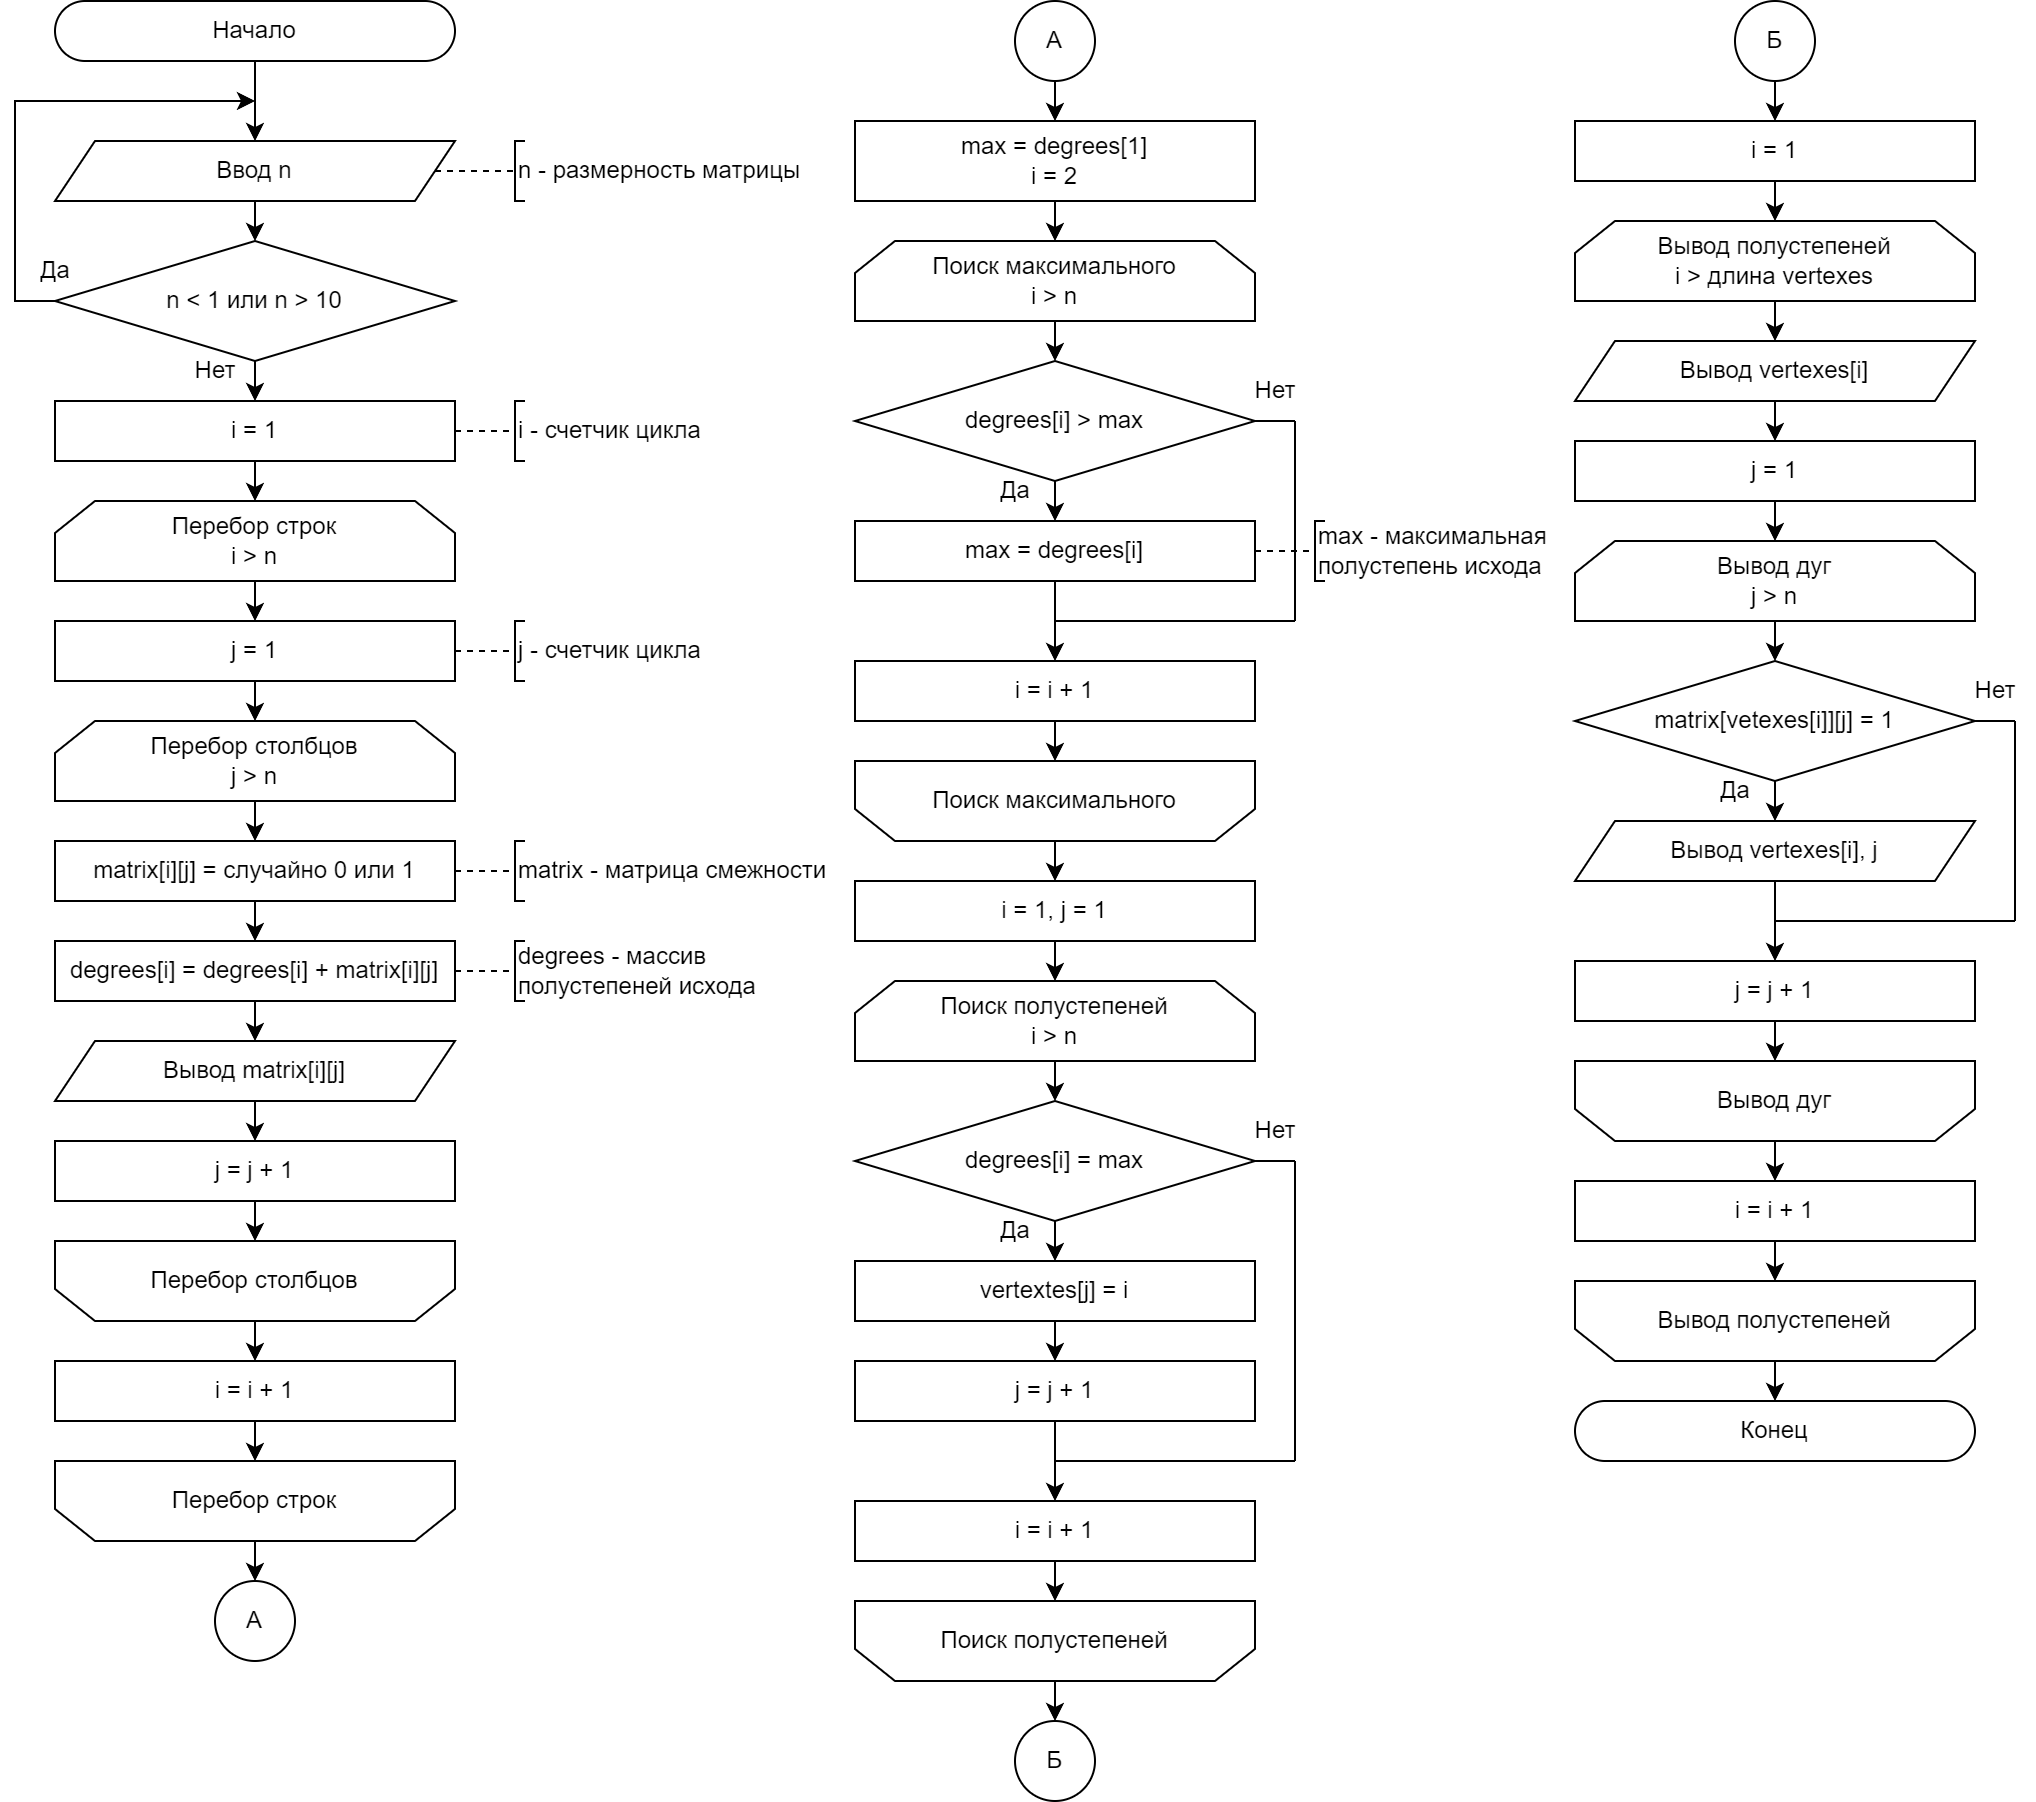
\includegraphics[width=1\linewidth]{images/scheme.png}
  \end{figure}
  \begin{center}
    Рисунок 1 – Схема алгоритма программы
  \end{center}

  При разработке реализована программа, исходный код которой представлен ниже.

  \begingroup
    \linespread{1}

    \begin{Verbatim}[tabsize=2]
var
  matrix: array[1..10, 1..10] of integer;
  degrees: array[1..10] of integer;
  vertexes: array[1..10] of integer;
  n, i, j, max: integer;

begin
  Randomize();

  repeat
    write('Введите размерность матрицы (4 <= n <= 10): ');
    readln(n);
  until (n >= 4) and (n <= 10);

  writeln('Матрица смежности', #10);

  write('  ');
  for i := 1 to n do
    write(' ', i, ' ');
  writeln();

  for i := 1 to n do
  begin
    write(i, '  ');
    for j := 1 to n do
    begin
      matrix[i][j] := Random(2);
      degrees[i] += matrix[i][j];
      write(matrix[i][j], '  ');
    end;
    writeln();
  end;
  writeln();

  max := degrees[1];

  for i := 2 to n do
  begin
    if (degrees[i] > max) then
      max := degrees[i];
  end;

  j := 1;

  for i := 1 to n do
  begin
    if degrees[i] = max then
    begin
      vertexes[j] := i;
      j := j + 1;
    end;
  end;

  writeln('Вершины с максимальной полустепенью исхода');

  i := 1;

  while vertexes[i] <> 0 do
  begin
    write('Множество дуг для вершины ', vertexes[i], ': {');
    for j := 1 to n do
    begin
      if matrix[vertexes[i]][j] = 1 then
        write(' (', vertexes[i], ', ', j, ')');
    end;
    writeln(' }');
    i := i + 1;
  end;

  readln;
end.
    \end{Verbatim}
  \endgroup

  Экранная форма программы в виде консольного приложения представлена на рисунке 2.
  \begin{figure}[h]
    \centering
    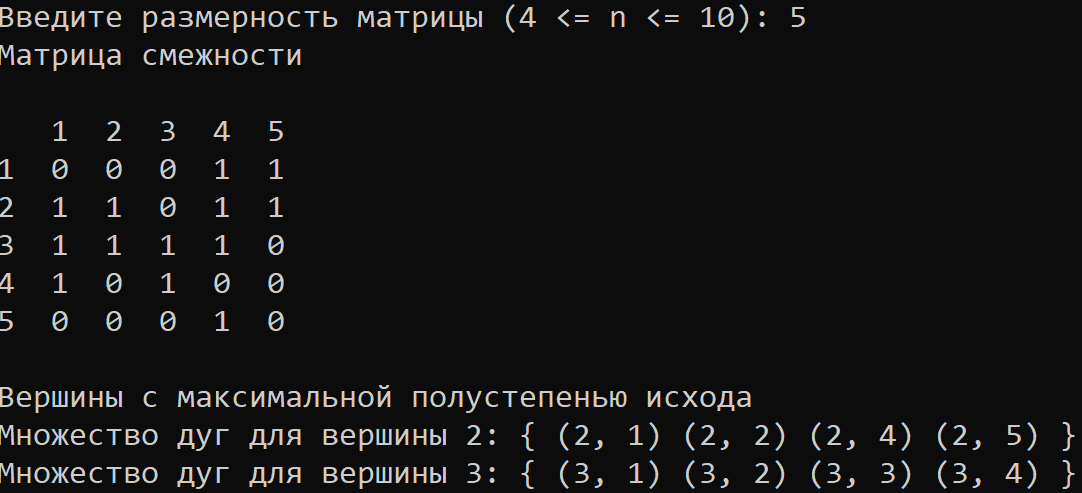
\includegraphics[width=0.8\linewidth]{images/image.png}
  \end{figure}
  \begin{center}
    Рисунок 2 – Консольный интерфейс программы
  \end{center}

  \section*{\hspace{12.5mm}Вывод}
  В процессе выполнения лабораторной работы, при решении предложенных задач, изучены основы теории графов и реализована программа на языке Паскаль, находящая номер вершины, имеющей максимальную полустепень исхода и выводит множество соответсвующих дуг в соответсвии матрицы смежности.

\end{document}